% M1 impact revision: matched fixed-score measurement, September 2026.
\RequirePackage{fix-cm}
\documentclass{article}
\usepackage{spconf,amsmath,graphicx,booktabs}
% Enforce the minimum also in mathematical subscripts and superscripts.
\DeclareMathSizes{9.1}{9.1}{9.1}{9.1}
\DeclareMathSizes{10}{10}{9.1}{9.1}
\renewcommand{\small}{\fontsize{9.1pt}{10.5pt}\selectfont}

\title{WHEN RESAMPLING CHANGES PAIRED DETECTOR COMPARISONS ON ASVSPOOF 2021 DF}
%
\name{\shortstack{Rafaello Virgilli \quad Lucas Alc\^antara Souza \quad Alexandre Costa Ferro Filho \quad Daniel Tunnermann\\[3pt]
Gustavo dos Reis Oliveira \quad Arlindo Rodrigues Galv\~ao Filho \quad Anderson da Silva Soares}}
\address{AKCIT, Federal University of Goi\'as (UFG), Goi\^ania, GO, Brazil\\
rafaello.virgilli@discente.ufg.br}

\begin{document}
\maketitle

\begin{abstract}\small
Comparing detectors on the same trials cancels shared variation, but does it remove sensitivity to which speakers and attacks receive weight? On fixed ASVspoof~2021~DF scores from eight detectors, we refit equal-error-rate (EER) thresholds under trial and joint speaker--attack resampling and construct simultaneous bands for all 28 EER differences. The number of bands excluding zero falls from 26 to 18. For XLSR-Mamba versus XLSR-Conformer, this occurs despite pairing removing about 75\% of summed marginal variance; the paired standard deviation increases 5.2-fold. A separate eleven-detector roster on the same corpus changes from 52 of 55 to 38 of 55 bands excluding zero. All sixteen comparisons between the four self-supervised detectors and four organizer baselines survive. These are sensitivity results for observed score collections, without population-coverage guarantees.
\end{abstract}

\begin{keywords}
Audio deepfake detection, paired evaluation, resampling, EER
\end{keywords}

\section{Introduction}
\label{sec:intro}
Does pairing detectors on the same trials cancel the effect of perturbing speakers and attacks? For HuBERT-ECAPA versus WavLM-ECAPA in Speech DF Arena \cite{shim25}, a $-2.153$-point EER gap has a trial-resampling band excluding zero, yet its joint speaker--attack band includes zero. XLSR-Mamba versus XLSR-Conformer shows the same change at $-0.389$ points (Fig.~\ref{fig:forest}). In both comparisons the scores and point gap stay fixed. What changes is the unit whose multiplicities vary.

ASVspoof~2021~DF has 533,928 evaluation trials but only 93 speakers and 110 attacks. Detectors can move together when an observed group gains weight, reducing the variation of their difference. Dependence in individual scores therefore does not by itself establish sensitivity of a paired EER contrast. The measurement question is which comparisons change when the perturbation unit changes while threshold refitting, system pairing and the comparison family are held fixed.

We measure whether paired detector comparisons survive changes in the resampling unit and in observed-group weights. The primary roster contains four author-released self-supervised (SSL) detectors and four organizer baselines; eleven Arena score files for the same trials form a separate roster. Named modern comparisons lose separation even after pairing cancels much of their marginal variation. One-factor perturbations and group deletions locate sensitivity within the observed 21DF score collection; a single-source SpoofCeleb check tests whether between-source reweighting is necessary. All sixteen SSL-versus-baseline comparisons survive the tested resampling laws and fixed weighting rules.

\section{Related work}
\label{sec:related}
\textbf{Benchmark reporting.} ASVspoof~2017 reported EER intervals \cite{delgado18}; ASVspoof~2021 Fig.~4(c) used the Bengio--Mari\'ethoz test \cite{bengio04} with Holm correction \cite{asvspoof21}. Its shared-trial variant accounts for two systems using the same trials, not repeated speakers and attacks. We found no uncertainty analysis in the later journal overview \cite{asvspoof21journal}, ASVspoof~5 \cite{asvspoof5eval}, or Arena report \cite{shim25}; a recent SSL benchmark reports point EERs \cite{spoofsuperb26}. Other work reports trial-bootstrap ranks \cite{xie26atadd}, EER spreads \cite{pascu24}, corrected pairwise tests \cite{martindonas24}, or fixed-threshold intervals \cite{weizman25}. Training-seed variation also moves rankings \cite{wang21_comparative}; our scores hold training fixed.

\textbf{Dependent paired comparison.} User-aware biometric and speech resampling \cite{poh07,wu17}, correlation-corrected paired tests \cite{wu16}, and synchronized resampling for correlated classifiers \cite{wukacker24} precede this study. Our speaker and spoof-attack factors are crossed \cite{cgm11,mccullagh00,owen07}, distinct from the nested-observation designs studied in \cite{anglin26}. The contribution is a matched measurement of paired EER comparisons under these perturbations, with every threshold refitted.

\textbf{Evaluation design.} Aggregation weights \cite{kwok25}, channel presentation \cite{delgado26presentation}, representations \cite{benchaudit26}, controlled generator/speaker perturbations \cite{pirlogeanu26} and corpus overlap \cite{stanek26} affect deepfake evaluation. Identity perturbations \cite{dar26}, speaker-adversarial training \cite{dao26} and speaker/synthesizer familiarity \cite{hong25twinshift} address related sensitivities. Here the scores are fixed and evaluation weights vary. Simultaneous rank intervals are established \cite{almohamad19}. Because selecting only neighbors in the observed point-EER ordering uses the outcomes, we include every detector pair.

\section{Method}
\label{sec:method}
\subsection{EER contrast and separation event}
\label{sec:eer}
Two deterministic systems on a fixed trial list have no sampling uncertainty until a perturbation law is declared. Scores are oriented so larger means bona fide and sorted in ascending order. At each ordered position, the false-reject rate (FRR) is the fraction of bona-fide weight at or below it and the false-accept rate (FAR) the fraction of spoof weight above it; we select the first position minimizing their absolute difference and take their mean as EER, without interpolation. For ordered pair $(A,B)$, $\Delta\mathrm{EER}_{A,B}=100(\mathrm{EER}_A-\mathrm{EER}_B)$ percentage points (negative favors $A$); every replicate refits both thresholds. A pair is \emph{separated under procedure $h$} when its simultaneous band excludes zero; write this indicator as $I_{p,h}$.

\subsection{Perturbation laws and scope}
The trial bootstrap independently resamples trials within class; for SpoofCeleb only, the archived plan samples the 91,130 trial indices from the pooled list with replacement, so class counts vary across replicates. In the speaker$\times$attack product-weight (PW) bootstrap \cite{owen07,oweneckles12}, we independently draw speakers and spoof attacks uniformly with replacement, drawing as many of each as observed; a spoof trial receives the product of its speaker and attack multiplicities, and a bona-fide trial receives only its speaker multiplicity. Speaker-only fixes attack multiplicities at one; attack-only fixes speaker and bona-fide trial weights at one. Each of these four procedures uses 5,000 replicates. Each replicate's weights are shared across systems; procedures have separate random streams.

\textbf{Interpretation.} These bands describe sensitivity of fixed scores to the stated weights, not confidence about future speakers or attacks. Four VCC spoof strata contain only 4, 4, 4 and 6 speakers. Coverage results for crossed-array means do not establish coverage for refitted EER differences \cite{oweneckles12}. The one-factor, Monte Carlo, mean/sign, pairing, tie and group-deletion diagnostics were designed after the primary results and are exploratory. Matching separation decisions does not decompose variance or identify a causal speaker effect. A band containing zero establishes neither equality nor a deployment ranking.

\subsection{All-pair simultaneous bands}
\label{sec:family}
For procedure $h$, let $s_{p,h}=\operatorname{sd}_b(\Delta_{p,h}^{(b)})$. We set $q_{.95,h}$ to the empirical 95th percentile of $\max_{p=1}^{28}|\Delta_{p,h}^{(b)}-\bar\Delta_{p,h}|/s_{p,h}$ and report $\hat\Delta_p\pm q_{.95,h}s_{p,h}$ \cite{montiel19}. The quantile centers deviations on the bootstrap mean, whereas the bands center on the original estimate; band inclusion is not an empirical reversal probability. The maximum includes all 28 primary contrasts, including when reporting within-cohort counts; Arena and SpoofCeleb use their own complete families. No population error-control guarantee is asserted. The historical independent- and shared-trial test reconstructions both separate five of six organizer pairs, without identifying the variant used in the published matrix.

\subsection{Alternative fixed weighting rules}
Within each class, every named hierarchy level receives equal conditional mass and trials divide their terminal-group mass equally. Bona-fide rules are empirical trial weights, equal mass over the three sources (ASVspoof, VCC2018, VCC2020), and equal source$\rightarrow$\allowbreak speaker mass. Spoof rules are empirical trial weights, equal mass over the five spoof strata (ASVspoof, VCC2018 HUB, VCC2018 SPO, VCC2020 Task~1, VCC2020 Task~2), equal mass over observed speaker$\times$attack cells within stratum, and equal mass successively over stratum, attack family (the attack-type field of the official 21DF trial metadata), attack and speaker. Their $3\times4$ crossing gives 12 positive, class-normalized rules fixed without inspecting scores.

\section{Experiments}
\label{sec:exp}
\textbf{Setup.} The primary set contains XLSR-Mamba \cite{xiao25}, XLS-R+SLS (SLS below) \cite{zhang24sls}, XLSR-Conformer \cite{rosello23} and SSL-AASIST \cite{tak22}, plus RawNet2, LFCC-LCNN, LFCC-GMM and CQCC-GMM. All 533,928 evaluation-phase trials have every score. The matched trial/PW comparison uses 5,000 replicates and seed 2026081604; seeds of the other analyses accompany their released outputs.

\textbf{Primary 21DF result.} The matched all-28-pair bootstrap refits the same weighted EER in every replicate. Trial and joint bands separate 26/28 and 18/28 pairs (Table~\ref{tab:eers}); within SSL, the counts fall from 5/6 to 2/6. Mamba--Conformer remains at $-0.389$ points: its trial band is $[-0.570,-0.208]$, its joint band $[-1.348,0.570]$. Speaker-only reproduces all eight joint losses; attack-only reproduces four or five of the eight joint losses across Monte Carlo repeats. All primary within-SSL losses involve Conformer.

Across five fresh attack-only runs, separation counts range from 21 to 22 overall and from two to three among organizer baselines; within-SSL counts remain three. For each other primary arm, 1,000 resamples of its saved 5,000 complete detector-output rows, recomputing all bands, leave every indicator unchanged. This assesses Monte Carlo noise conditional on saved draws, not independent-seed stability. Five fresh 5,000-draw runs for each of the trial, speaker-only and joint arms also preserve every recorded separation indicator.

\textbf{Arena comparison.} On the eleven complete Speech DF Arena score files for the same 533,928 trials, trial and PW bands separate 52/55 and 38/55 pairs. For HuBERT-ECAPA versus WavLM-ECAPA, the $-2.153$-point gap has bands $[-2.761,-1.544]$ and $[-5.241,0.936]$. Its joint pointwise percentile interval remains below zero, [$-4.252$, $-0.277$]; the loss is specifically under the 55-pair simultaneous band.

\begin{table}[tb]
\caption{Top: primary 21DF EER (\%), with 14,869 bona-fide and 519,059 spoof trials and weights normalized within class. Middle: paired bands in percentage points; primary 21DF uses all 28 pairs, Arena all 55 pairs. Bottom: primary separation counts, retaining the 28-pair correction; every arm retains 16/16 SSL-versus-baseline separations. Attack ranges span the original and five fresh 5,000-draw runs; other entries are recorded-run counts. Primary Monte Carlo checks are described in the text. One-factor analyses are exploratory.}
\label{tab:eers}
\centering\small
\vspace{2pt}
\begin{tabular}{@{}lccc@{}}
\toprule
SSL detector & EER & Organizer baseline & EER \\
\midrule
XLSR-Mamba & 1.884 & RawNet2 & 22.383 \\
XLS-R+SLS & 1.916 & LFCC-LCNN & 23.477 \\
XLSR-Conformer & 2.273 & LFCC-GMM & 25.247 \\
SSL-AASIST & 2.852 & CQCC-GMM & 25.563 \\
\midrule
\multicolumn{4}{@{}l@{}}{XLSR-Mamba $-$ XLSR-Conformer: $-0.389$} \\
\multicolumn{2}{@{}l}{Trial $[-0.570,-0.208]$} & \multicolumn{2}{l@{}}{PW $[-1.348,0.570]$} \\
\multicolumn{4}{@{}l@{}}{Arena HuBERT-ECAPA $-$ WavLM-ECAPA: $-2.153$} \\
\multicolumn{2}{@{}l}{Trial $[-2.761,-1.544]$} & \multicolumn{2}{l@{}}{PW $[-5.241,0.936]$} \\
\bottomrule
\end{tabular}

\smallskip
\setlength{\tabcolsep}{3pt}
\begin{tabular}{@{}lcccc@{}}
\toprule
Roster / subset & Trial & Speaker & Attack & Joint \\
\midrule
21DF, all & 26/28 & 18/28 & 21--22/28 & 18/28 \\
21DF, SSL & 5/6 & 2/6 & 3/6 & 2/6 \\
21DF, organizer & 5/6 & 0/6 & 2--3/6 & 0/6 \\
\bottomrule
\end{tabular}
\end{table}

\begin{figure}[t]
\centering
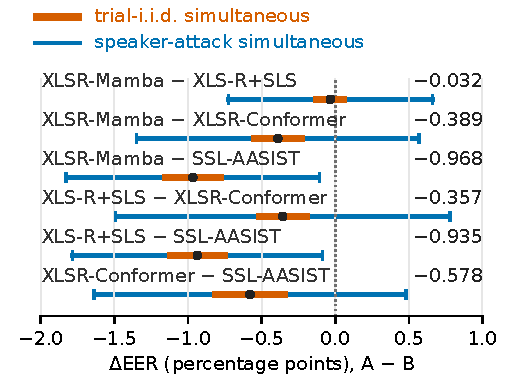
\includegraphics[width=\columnwidth]{figs/forest.pdf}
\caption{All six within-SSL pairs on primary 21DF. Dots and right-hand labels are point gaps ($A-B$; negative favors $A$). Thick orange: trial bands; thin blue with end caps: PW bands. Both retain the full 28-pair simultaneous max-$t$ construction. Five trial bands and two PW bands exclude zero; the point estimates do not change.}
\label{fig:forest}
\end{figure}

\textbf{Pairing and band interpretation.} Under the joint law, Mamba and Conformer EERs correlate 0.777; pairing removes about 75\% of the sum of their marginal variances, yet the paired SD rises from 0.06149 under trials to 0.31997 points under joint resampling. Table~\ref{tab:sign} distinguishes mean displacement, sign frequency and band separation. The joint mean displacement is only 0.032 SD, so band centering does not explain inclusion of zero; the trial band excludes zero with 0/5,000 opposite-sign draws, the joint band includes it with 463/5,000.

\begin{table}[t]
\caption{Mamba minus Conformer: mean shift from the point gap, pair SD (points), opposite-sign draws out of 5,000, and zero exclusion under the full 28-pair band.}
\label{tab:sign}
\centering\small
\setlength{\tabcolsep}{4pt}
\begin{tabular}{@{}lrrrr@{}}
\toprule
Law & Mean shift & SD & Opposite & Excludes? \\
\midrule
Trial & $-0.002492$ & 0.061488 & 0 & Yes \\
Speaker & $-0.003175$ & 0.270826 & 210 & No \\
Attack & $-0.010235$ & 0.147333 & 37 & No \\
Joint & $-0.010135$ & 0.319971 & 463 & No \\
\bottomrule
\end{tabular}
\end{table}

\textbf{Observed-group influence.} Deleting VCC2SM3, which contains 315 bona-fide VCC2018 trials and no spoof trials, changes the Mamba--Conformer gap from $-0.389$ to $-0.129$ percentage points. This locates influence in an observed genuine-speech group; it does not identify a causal speaker effect.

\textbf{Composition-preserving control.} A post-result PW control resamples speakers and attacks within each bona-fide source or spoof stratum, rejects draws with no class support in any required stratum, and rescales the three bona-fide source masses and five spoof-stratum masses to their observed values. Across 1,000 retained draws it separates 18/28 pairs and 0/6 organizer pairs. Thus movement of these eight masses is not required for the loss of separation; this does not remove influence from groups within a source or stratum.

\textbf{Check on single-source SpoofCeleb.} On all 91,130 SpoofCeleb evaluation trials \cite{jung25spoofceleb}, pooled trial resampling separates 6/6 pairs and joint resampling 3/6; class-stratified trial resampling also gives 6/6. EERs are 57.93\%, 24.51\%, 26.72\% and 27.58\% for AASIST, SLS, SSL-AASIST and Mamba. Under the original six-pair correction, all three comparisons among SLS, SSL-AASIST and Mamba lose separation; the three AASIST contrasts retain it. Every base item has one bona-fide and nine spoof renditions under one source label, so between-source mass cannot change. This is a control on a weakly transferred, off-domain roster, not evidence that attack effects generally dominate speaker effects on another corpus.

\textbf{Alternative weights.} Fixed rules reverse 5/6 organizer-baseline, 1/6 within-SSL and 0/16 cross-cohort point orderings. The SSL pair is Mamba--SLS (gap $-0.032$ points), already unseparated under trial resampling. Recomputing both bootstraps with each rule's weights as base weights (computed after the primary results, 5,000 draws per rule and bootstrap) separates all 16 cross-cohort pairs in all 24 rule$\times$law cells; the closest band endpoint to zero is $-12.79$ points.

\clearpage
\section{Discussion}
\label{sec:disc}
\textbf{Reporting decision rule.} For comparisons intended to withstand changes in the weights of observed speakers and attacks, report the point EER difference and both trial and group-resampling bands for the same comparison family. If only the trial band excludes zero, report that separation depends on the resampling law; do not infer equality or population significance from the group band. Publish the group memberships and weighting rules needed to reproduce the check.

\textbf{Coverage boundary.} In a separate simulation using the 21DF incidence and Gaussian speaker/attack effects fitted to RawNet2/LFCC-LCNN scores, nominal 95\% pointwise percentile intervals covered a true 0.5-point EER difference in 37/200 datasets (18.5\%) under trial resampling and 196/200 (98.0\%) under speaker$\times$attack resampling, using 300 bootstrap draws per dataset. In a separate 24-cell low-EER grid varying interaction strength, effect tails and the true gap, speaker$\times$attack percentile coverage fell below 90\% in 11 cells, reaching 85.5\% (1,000 datasets per cell; 500 bootstrap draws). These models have not been validated for 21DF, and these pointwise intervals differ from our all-pair bands; neither result establishes coverage for those bands.

\newpage
\begingroup\raggedright
\textbf{Artifact.} Code, score provenance, complete numerical results and additional reproducibility checks are available in the public artifact. Artifact version \texttt{4ee170b035f46097832f0973aff534418fc54157} at \mbox{github.com/rvirgilli/asvspoof2021-df-clustered-uncertainty}.\par\endgroup

\section{Conclusion}
On the observed ASVspoof~2021~DF scores, changing the resampling unit changes paired EER separation even after substantial variation cancels between detectors. Mamba--Conformer illustrates this with about 75\% covariance cancellation and a 5.2-fold increase in paired standard deviation. The sixteen SSL-versus-baseline contrasts survive the tested resampling laws and fixed weighting rules. These results support reporting sensitivity to observed-group weights, without establishing population confidence or a universal factor pattern across corpora.

\section{Acknowledgment}
During preparation, the authors used large language models (Anthropic Claude and OpenAI Codex) to help edit the text, LaTeX layout and supporting code. The authors reviewed all assisted content and take full responsibility.

\section{Compliance with Ethical Standards}
This study analyzed previously collected ASVspoof~2021 and SpoofCeleb recordings and detector scores. It involved no new recording or interaction with human participants; no ethical approval was required. The authors declare no competing interests.

\clearpage
\let\oldthebibliography\thebibliography
\renewcommand{\thebibliography}[1]{\oldthebibliography{#1}%
  \setlength{\itemsep}{0pt}\setlength{\parsep}{0pt}\setlength{\parskip}{0pt}\setlength{\topsep}{2pt}}
{\small
\bibliographystyle{IEEEbib}
\bibliography{refs}
}
\end{document}
